\documentclass[aspectratio=169]{beamer}
\usepackage[portuguese]{babel}
\usepackage{xcolor} % Para colorir o código
\usepackage{booktabs} % Para a formatação da tabela
\usepackage{array}    % Para a personalização de colunas
\usepackage{pgfplots} % Pacote para gráficos
\usepackage{amsmath}
\usepackage{graphicx}

\usetheme{DarkConsole}

\title{Precificação de ativos de renda variável}
\subtitle{Uma Abordagem Baseada em Dados Históricos}
\author{\\Cauã Wendel Sousa da Silva \\ Hertz Rafael Queiroz da Cruz}

\begin{document}

% Slide de título
\begin{frame}
  \maketitle
\end{frame}


% Sumário
\begin{frame}{Sumário}
  \tableofcontents
\end{frame}

% Introdução
\section{Introdução}
\begin{frame}{Introdução}

  \begin{center}
    {\Large Como identificar quais os melhores ativos a serem investidos através de dados estatísticos?}

    
  \end{center}

  \vspace{0.5cm}
Neste trabalho, buscamos responder a essa questão utilizando métodos estatísticos que permitem analisar tendências e históricos de ações, a fim de auxiliar o investidor na tomada de decisões.


  
\end{frame}

\begin{frame}{Introdução}

  \begin{itemize}
    \item "A população brasileira, em geral, não tem a cultura de organizar suas finanças e tampouco de poupar recursos." \cite{Mendes2015}
    \item "O desequilíbrio financeiro e a falta de disciplina são os principais fatores negativos para a atual situação." \cite{Mendes2015}
    \item Dessa forma, grande parte da população do Brasil atualmente não possui sequer a capacidade financeira ou intelectual de realizar investimentos em ativos e, ainda que em casos mais incomuns, preferem investir em renda fixa, que oferece um menor risco, porém comprometendo sua rentabilidade quando comparada à renda variável.
  \end{itemize}
  
\end{frame}

% Revisão da Literatura
\section{Revisão da Literatura}
\begin{frame}{Revisão da Literatura}
  \begin{itemize}
    \item Ativos de Renda Variável: São aqueles cujo retorno não é fixo ou garantido, variando conforme as condições de mercado, como ações e alguns fundos de investimentos.

    \item Oferecem maior potencial de retorno, porém com maior risco.

    \item Para proteção do investidor, a 'Modern Portfolio Theory'
    de Markowitz (1952) surge como uma estrutura de investimento para a seleção e
    construção de carteiras de investimentos com base na maximização dos retornos esperados da carteira e a minimização simultânea do risco de investimento. \cite{mangram2013simplified}
    
  \end{itemize}
\end{frame}

\begin{frame}{Revisão da Literatura}
  \begin{itemize}
    \item Índice de Sharpe: Avalia a relação entre risco e retorno, levando em consideração uma taxa livre de risco. Esse índice fornece ao investidor a informação necessária para determinar se os riscos de possíveis perdas são compensados pelo retorno esperado. \cite{de2015fundos}

    \item Bandas de Bollinger: Serve para identificar quando o investidor deve comprar ou vender suas ações a fim de maximizar seus lucros, comprando enquanto está desvalorizado e vendendo supervalorizado. \cite{yan2023enhanced}

    \item Desvio Padrão: Caracteriza a distância típica de uma observação do centro da distribuição; em outras palavras, reflete a dispersão das observações individuais da amostra em torno da média da amostra. \cite{curran1998fundamental}

    \item Média Móvel: Resume os padrões gerais de mudança ao longo de um período passado e é frequentemente utilizada para prever a tendência futura de séries temporais. \cite{su2022self}

  \end{itemize}
\end{frame}

% Objetivos
\section{Objetivos}
\begin{frame}{Objetivos}
  \textbf{Geral:}  
  Obter insights que possam ajudar o investidor a identificar em qual ativo pode ser mais rentável investir, com base em dados históricos e estatísticas.

  \vspace{0.5cm}
  \textbf{Específicos:}
  \begin{itemize}
    \item Utilizar o Índice de Sharpe para comparar o retorno ajustado ao risco entre diferentes investimentos.
    \item Calcular a Média Móvel para identificar tendências de preço ao longo do tempo.
    \item Aplicar as Bandas de Bollinger para detectar condições de valorização ou desvalorização nos ativos.
  \end{itemize}
\end{frame}

% Metodologia
\section{Metodologia}
\begin{frame}{Metodologia}
  \textbf{Ferramentas e Procedimentos Utilizados:}
  \begin{itemize}
    \item Coleta de dados financeiros via biblioteca do \texttt{yfinance}.
    \item Transformação e limpeza dos dados do DataFrame utilizando \texttt{pandas}, incluindo padronização das colunas.
    \item Consideração do retorno sobre o risco através do Índice de Sharpe.
    \item Utilização da Média Móvel para identificar a tendência do valor de um ativo.
    \item Aplicação das bandas de Bollinger para avaliação de valorização ou desvalorização dos ativos.
    \item  Criação de gráficos na biblioteca \texttt{plotly}
    \item Desenvolvimento de um aplicativo web na biblioteca \texttt{streamlit}
  \end{itemize}
\end{frame}

\section{Aplicativo}
\begin{frame}{Funcionalidades do Aplicativo}
  \begin{itemize}
    \item \textbf{Histórico de Preços:}
    \begin{itemize}
      \item Coleta do histórico de preços e plotagem em um gráfico interativo utilizando \texttt{Plotly}.
      \item Exibição das seguintes métricas: valor inicial, valor mínimo, valor médio, valor máximo e valor atual.
    \end{itemize}

    \item \textbf{Retorno Acumulado:}
    \begin{itemize}
      \item Cálculo do retorno acumulado e visualização em um gráfico interativo usando \texttt{Plotly}.
      \item Exibição das métricas: retorno acumulado médio, menor retorno, maior retorno e retorno acumulado total.
    \end{itemize}

    \item \textbf{Índice de Sharpe Mensal:}
    \begin{itemize}
      \item Cálculo do Índice de Sharpe por mês, avaliando a relação risco/retorno.
      \item Exibição de um \texttt{DataFrame} com os valores mensais no \texttt{Streamlit}.
    \end{itemize}

    \item \textbf{Bandas de Bollinger:}
    \begin{itemize}
      \item Cálculo das Bandas de Bollinger e plotagem em gráfico interativo com \texttt{Plotly}.
      \item Exibição das métricas: maior valor, menor valor, valor médio e desvio padrão no período.
    \end{itemize}
  \end{itemize}
\end{frame}

\section{Demonstração do Aplicativo}
\begin{frame}{Exibir Gráfico do Histórico}
    \begin{figure}
        \centering
        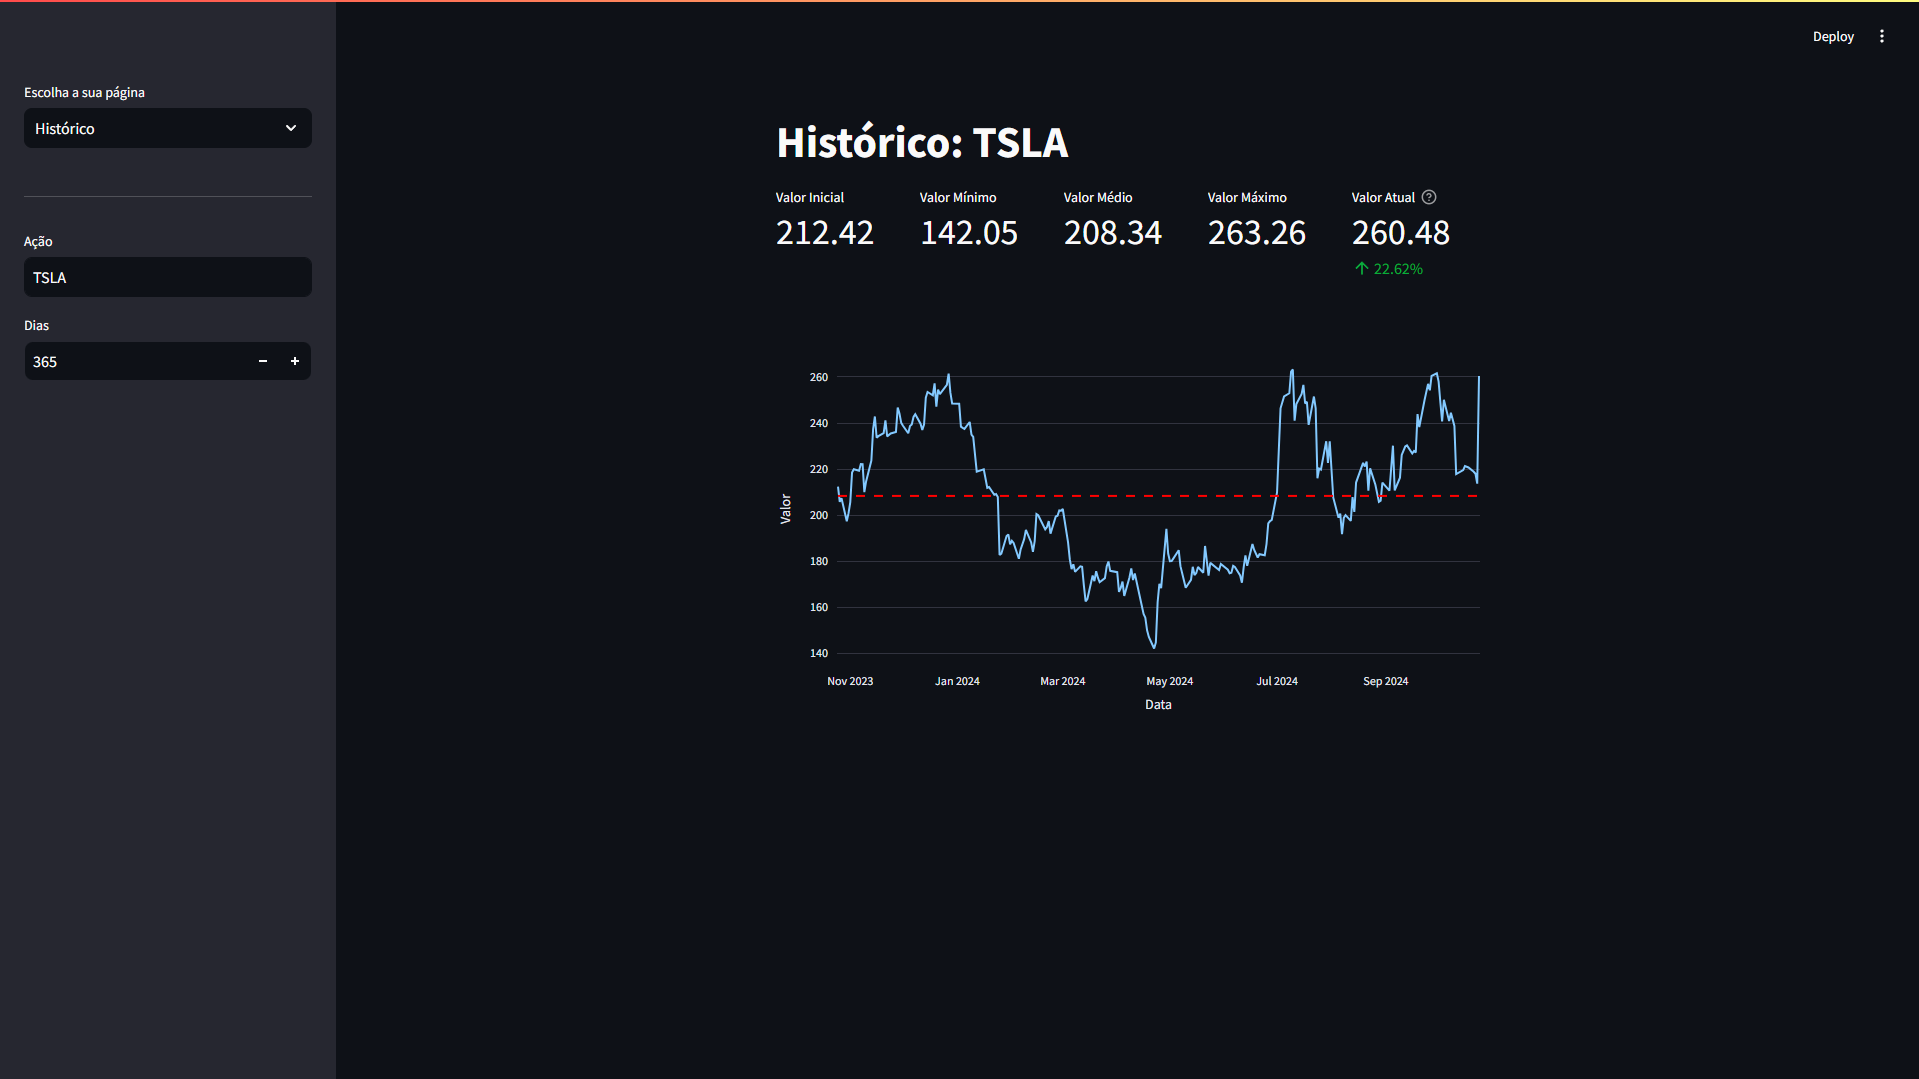
\includegraphics[width=0.8\textwidth]{F1.png}
    \end{figure}
\end{frame}

\begin{frame}{Exibir Gráfico do Retorno Acumulado}
    \begin{figure}
        \centering
        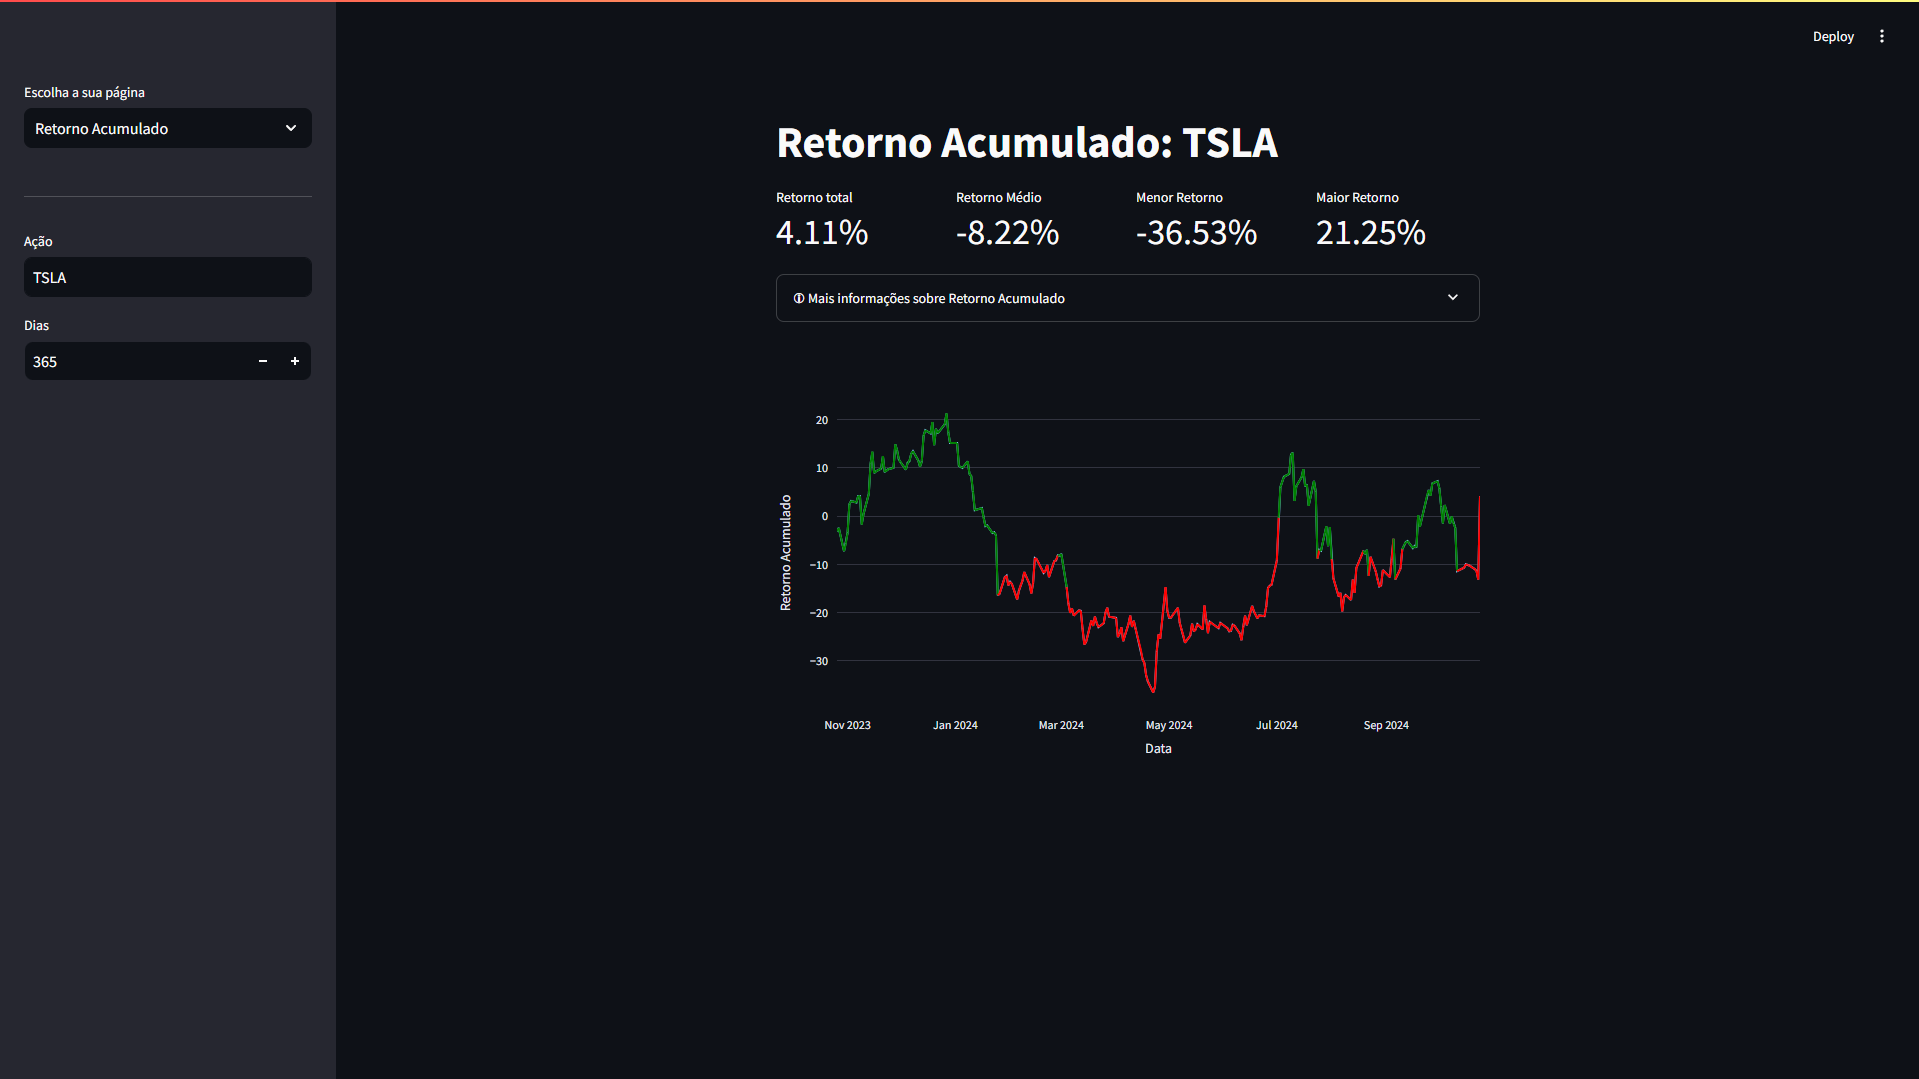
\includegraphics[width=0.8\textwidth]{F2.png}
    \end{figure}
\end{frame}

\begin{frame}{Exibir Dataframe do Índice de Sharpe}
    \begin{figure}
        \centering
        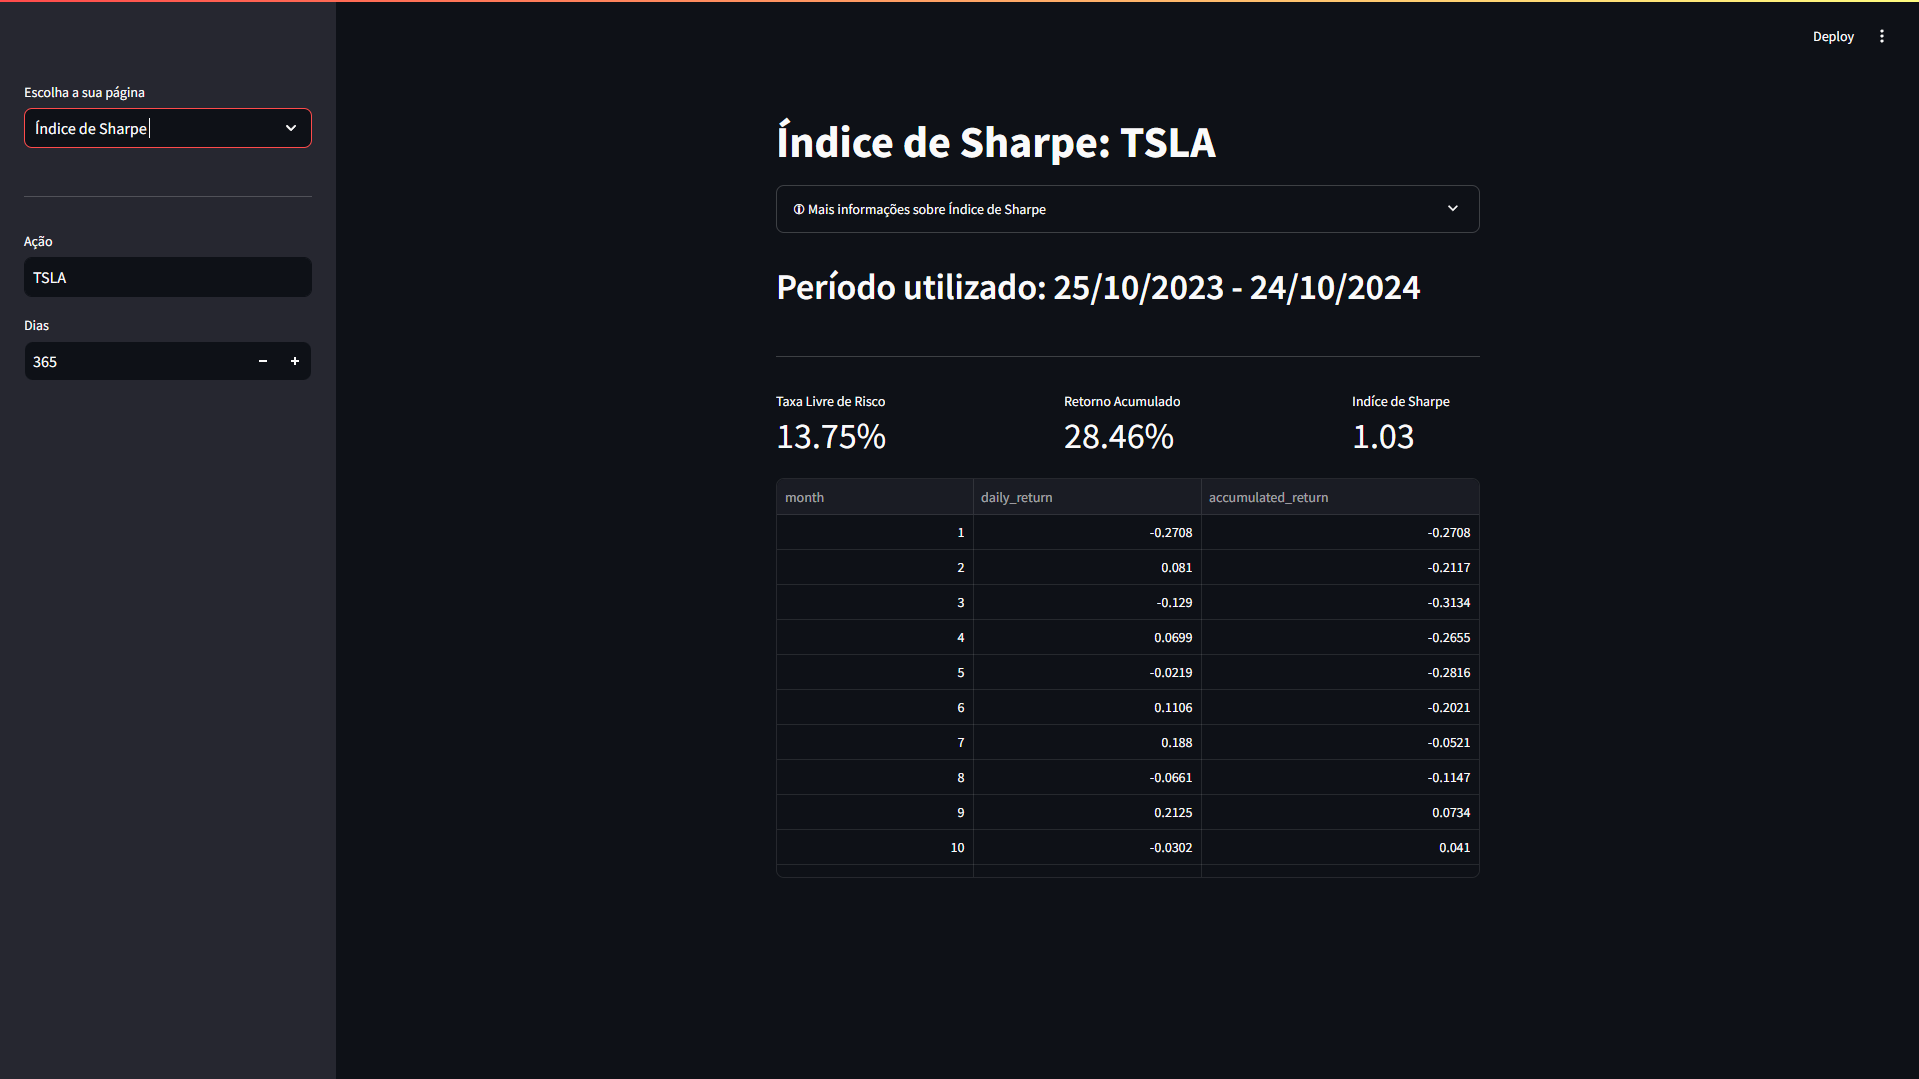
\includegraphics[width=0.8\textwidth]{F3.png}
    \end{figure}
\end{frame}

\begin{frame}{Exibir Gráfico das Bandas de Bollinger}
    \begin{figure}
        \centering
        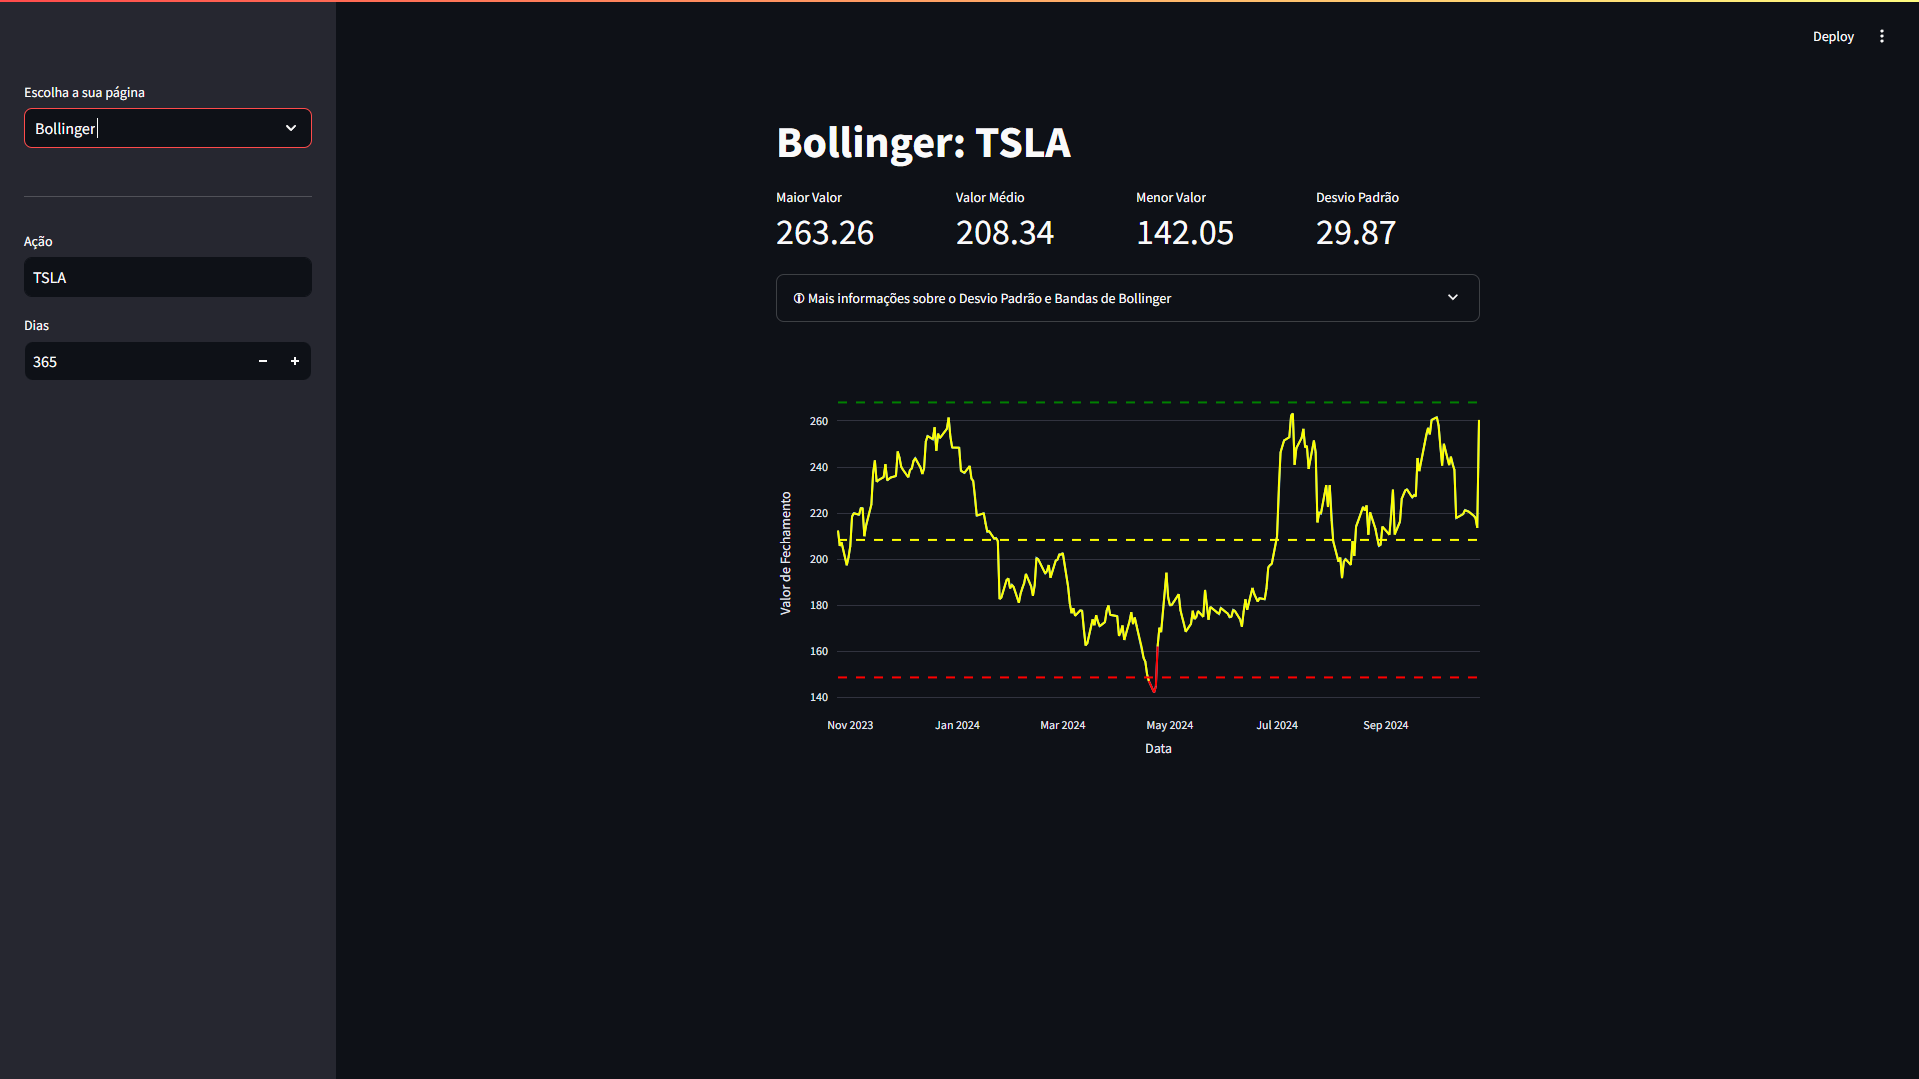
\includegraphics[width=0.8\textwidth]{F4.png}
    \end{figure}
\end{frame}

% Conclusão
\section{Conclusão}
\begin{frame}{Contribuição do Trabalho}
  Este trabalho apresenta uma abordagem estatística que permite ao investidor extrair insights valiosos com base em dados históricos e tendências. Utilizando métodos como o Índice de Sharpe, a Média Móvel e as Bandas de Bollinger é possível que o usuário tome decisões mais informadas e aumente suas chances de identificar ativos com maior potencial de rentabilidade.
\end{frame}

\bibliographystyle{plain}
\bibliography{ref}
\end{document}